 \documentclass[a4paper,10pt]{article}
\input{/Users/WannaGetHigh/workspace/latex/macros.tex}

\title{M3DA - TP 2 : mise en correspondance st\'er\'eoscopique}
\author{Fran\c cois \bsc{Lepan}}

\begin{document}
\maketitle

\section*{Introduction}

Dans ce rapport nous allons voir comment faire pour reconstruire en 3D certains points d'une sc\`ene \`a partir de deux images de cette sc\`ene poss\'edant un point de vue diff\'erent. \\

Pour ce faire nous allons passer par plusieurs \'etapes :
 
\begin{itemize}
\item le calcul de la matrice fondamentale,
\item l'extraction des "coins",
\item le calcule des distances,
\item Et enfin il faut faire la mise en correspondance des points des deux images.
\end{itemize}

\section{Calcul de la matrice fondamentale}

La matrice fondamentale est une matrice qui permet de passer d'un point d'une image de la sc\`ene \`a une droite sur l'autre image de cette sc\`ene appel\'e droite \'epipolaire. 

\begin{figure}[ht]
\begin{center}
	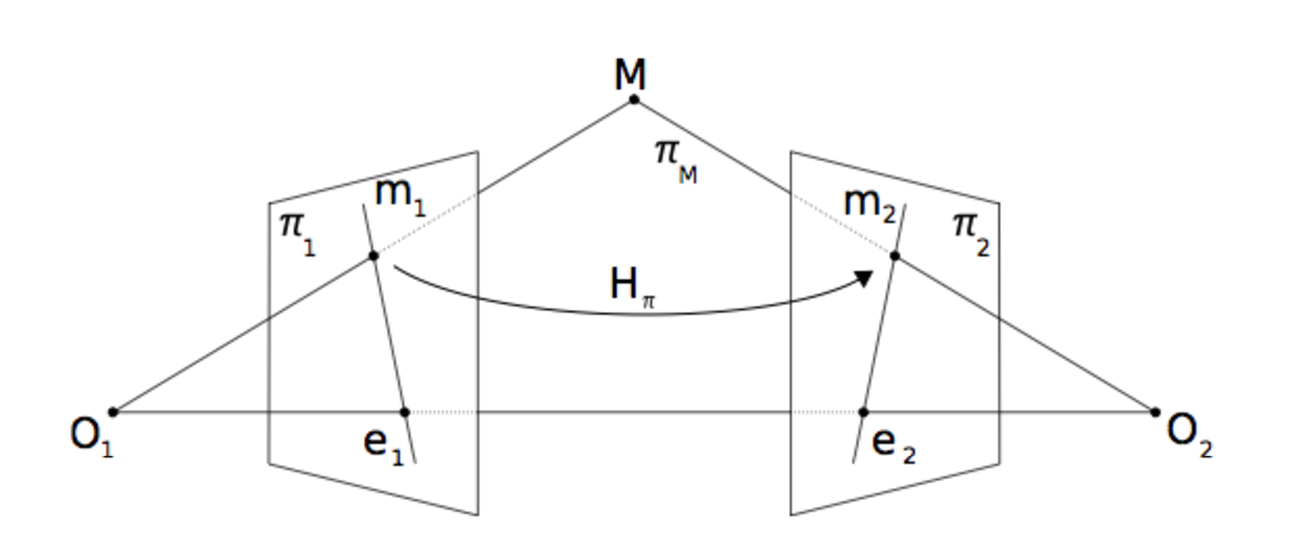
\includegraphics[width=10cm]{images/matrice_fondamentale.pdf}
\end{center}
	\caption{Sch\'ema matrice fondamentale}
	\label{matrice_fond}
\end{figure}

Sur la ~Fig.~\ref{matrice_fond}  la matrice fondamentale $F$ est la matrice qui permet de passer du point $m_1$ \`a la droite $e_2m_2$.

Cette matrice nous donnant pour un point de l'image de gauche une droite \'epipolaire sur l'image de droite (et inversement) il va falloir d\'eterminer quel point sera le meilleur candidat.

Pour ce faire nous allons voir comment tout d'abord trouver des points particulier permettant de facilement les mettre en correspondance sur chaque image.

\section{Extraction des coins}

Afin de mettre en correspondance pixels d'int\'er\^et dans les deux images nous allons extraire les "coins" gr\^ace \`a une m\'ethode propos\'e par \emph{Jianbo Shi et Carlo Tomasi} en 1994. On appel ces pixels d'int\'er\^et "coins" car ils correspondent principalement aux pixels situ\'es \`a l'intersection de deux lignes de pixels d'une m\^eme couleur.

Pour ce faire nous utiliserons une m\'ethode de la librairie openCV appel\'e \emph{goodFeaturesToTrack} qui s'occupe de trouv\'e ces coins.

\begin{Verbatim}[commandchars=\\\{\}]
void goodFeaturesToTrack(InputArray image, 
			OutputArray corners, 
			int maxCorners, 
			double qualityLevel, 
			double minDistance, 
			InputArray mask=noArray(), 
			int blockSize=3, 
			bool useHarrisDetector=false, 
			double k=0.04 )
\end{Verbatim}

Cette m\'ethode prend en param\`etre une image \`a analyser, un tableau \`a remplir, une distance minimum entre chaque points trouv\'e et d'autres param\`etres permettant d'affin\'e la recherche.

Apr\`es utilisation de cette m\'ethode on se retrouve avec nos points d'int\'er\^ets pour chaque images. Reste la mise en correspondance entre les points de l'image de gauche et l'image de droite.

\section{Calcul des distances}

Une premi\`ere \'etape de mise en correspondance consiste \`a calculer les distances :
 \begin{itemize}
 \item pour chaque droites \'epipolaires issue des points de l'image de gauche les distances entre ces droites et tous les points de l'image de droite que l'on va stocker dans une matrice m1, \\
\item pour chaque droites \'epipolaires issue des points de l'image de droite les distances entre ces droites et tous les points de l'image de gauche que l'on va stocker dans une matrice m2, \\
\item enfin il ne reste qu'a additionner chaque distance D correspondante : $m = m1*m2^t$.
 \end{itemize}
~\\

Explication pour deux points quelconque :

\begin{Verbatim}[commandchars=\\\{\}]
A point image de gauche.
B point image de droite.
Ad droite \'epipolaire du point A
Bd droite \'epipolaire du point B

d1 = distance entre A et Bd
d2  = distance entre B et Ad

d = d1 + d2;
\end{Verbatim}

Maintenant que nous avons les distances il ne reste qu'a trouver les correspondances entre ces points.

\section{Mise en correspondance}

La mise en correspondance consiste \`a dire qu'un point A de l'image de gauche \`a le plus de chance d'\^etre un point B de l'image de droite. \\

Pour ce faire nous allons proc\'eder de la fa\c con suivante :

\begin{Verbatim}[commandchars=\\\{\}]
\codeBlue{// mDistances = matrice des distances}
\codeBlue{// dMaxDistance = distance maximale autorisant une association}

\codeBlue{// nombre de tour a effectuer}
int nbTurn = 0;
int index = 0;

\codeBlue{// ces deux listes sont initialisee avec des -1}
\codeBlue{// liste des correspondants des points gauche}
mRightHomologous = initMatrix(mDistances.cols);
\codeBlue{// liste des correspondants des points droite}
mLeftHomologous = initMatrix(mDistances.rows);

\codeBlue{// calcule du nombre d'association a effectuer :}
\codeBlue{// le plus petit nombre de point trouve pour une image}
\codeBlue{// car on ne peut avoir qu'une association par point }
if (mDistances.rows > mDistances.cols)  
	nbTurn = mDistances.cols;
else                                    
	nbTurn = mDistances.rows;

\codeBlue{// les indices des points a associer}
int x;
int y;

\codeBlue{// tant qu'il reste des points a associer}
while (index < nbTurn) \{
	\codeBlue{// si on a trouv\'e une association}
	if (findMinValue(mDistances,x,y,dMaxDistance)) \{
	\codeBlue{// on associe les points}
	mRightHomologous.at<int>(x) = y;
	mLeftHomologous.at<int>(y) = x;
	\codeBlue{// on emp\^eche d'autres association pour ces deux points}
	removeLigneColFrom(mDistances,x,y);
	\}
	index++;
\}
\end{Verbatim}

\`A la sortie de cette algorithme on obtient deux vecteur contenant pour chaque point son correspondant et si ce point n'a pas de correspondant alors on \`a la valeur -1.

\newpage

Example :

\begin{Verbatim}[commandchars=\\\{\}]
mRightHomologous = [4; -1; 1; 9; 3; -1; 5; 7; -1; 8]
mLeftHomologous =  [-1; 2; -1; 4; 0; 6; -1; 7; 9; 3]
\end{Verbatim}

\section*{Conclusion}

Cette m\'ethode de mise en correspondance st\'er\'eoscopique via l'analyse de point d'int\'er\^ets des deux images fonctionne correctement. Mais notre approche peut \^etre am\'elior\'ee car on ne prend que la position g\'eom\'etrique des points. On pourrait prendre la colorim\'etrie des images afin d'affiner la recherche de correspondant.

\end{document}